\documentclass[11pt]{article}
\usepackage[margin=1in]{geometry}
\usepackage{amsmath,amssymb,amsthm}
\usepackage{booktabs}
\usepackage{hyperref}
\usepackage{microtype}
\usepackage{parskip}
\usepackage{xcolor}
\usepackage{algorithm}
\usepackage{algpseudocode}
\usepackage{graphicx}
\usepackage{natbib}
\usepackage{enumitem}

\newtheorem{theorem}{Theorem}
\newtheorem{proposition}{Proposition}
\newtheorem{remark}{Remark}
\newtheorem{definition}{Definition}

\title{Spatially-Coupled Generative Deconvolution via\\the Moran Stochastic Bridge}
\author{Ho Lung Tsui}
\date{\today}

\begin{document}
\maketitle

%% ==================================================================
\begin{abstract}
%% ==================================================================
Spatial transcriptomics technologies such as Visium and MERFISH measure gene expression at tissue-spot resolution, but each spot aggregates counts from tens of cells, obscuring the single-cell heterogeneity critical for understanding tissue architecture. We introduce the \textbf{Moran Bridge}, a spatially-coupled generative framework that deconvolves these aggregated measurements into per-cell expression profiles. Drawing on classical population genetics, we model cells within each spot as a finite population evolving under a Moran continuous-time Markov chain (CTMC), combining per-gene immigration--death mutation with inter-cell resampling weighted by a Gaussian spatial kernel. At stationarity, this process converges to a Dirichlet Process mixture---a principled nonparametric prior over cell-type compositions. Generation proceeds by reversing the CTMC from this prior using Anderson's theorem, guided by a permutation-equivariant DeepSets denoiser trained via Expectation--Maximisation with an $L^2$-squared Chamfer loss. Applied to the Vizgen Mouse Brain MERFISH dataset (78{,}329 cells, 649 genes), the 3.8M-parameter Moran Bridge achieves a $2.5\times$ improvement in Wasserstein distance and $7.1\times$ improvement in variance error over the 100.5M-parameter Count Bridge baseline under identical compute budgets, demonstrating that physically-grounded spatial priors can dramatically improve both accuracy and efficiency in spatial deconvolution.
\end{abstract}

%% ==================================================================
\section{Introduction}
\label{sec:intro}
%% ==================================================================

The rapid development of spatially-resolved transcriptomics has transformed our ability to study gene expression \emph{in situ}, preserving the spatial context that is lost in dissociated single-cell assays~\citep{moses2022museum}. Technologies such as Visium~\citep{stahl2016visium} and MERFISH~\citep{vizgen2021merfish} now routinely profile thousands of genes across tissue sections. However, many of these platforms measure expression at \emph{spot} resolution, where each spot aggregates the transcripts of anywhere from a handful to dozens of cells. Recovering the individual cell profiles from these aggregates---the \emph{spatial deconvolution} problem---is essential for mapping cellular heterogeneity, identifying rare cell types, and understanding cell--cell communication within tissues.

Existing deconvolution methods fall into two broad categories. \emph{Reference-based} approaches such as cell2location~\citep{kleshchevnikov2022cell2location} and RCTD~\citep{cable2022rctd} leverage external single-cell RNA-seq atlases to estimate cell-type proportions per spot, but they cannot recover full count profiles and require matched reference datasets that may not exist for the tissue of interest. \emph{Reference-free} methods such as STdeconvolve~\citep{miller2022stdeconvolve} operate without external data but are limited to cluster-level proportion estimates rather than per-cell count vectors.

Recently, \citet{fishman2025count} introduced \emph{Count Bridges}, a stochastic bridge process on the integers that extends diffusion-style generative models to count data. Using a multimodal U-ViT architecture with 100M parameters, they demonstrated that a generative model trained via EM can produce per-cell count profiles directly from spot-level aggregates---the first reference-free method to do so. However, their approach treats cells within each spot as \emph{independent} conditional on the aggregate, ignoring the spatial structure that governs how cell types organize in tissue. This independence assumption, combined with the massive parameter count, leads to mode collapse: the authors themselves reported that CellTypist identified only 26 cell types in their generated profiles versus 278 in the ground truth.

We propose a fundamentally different approach rooted in \textbf{population genetics}. Rather than treating cells independently, we model them as a finite population evolving under a \emph{Moran process}~\citep{moran1958random}---a continuous-time Markov chain that couples cells through spatially-weighted resampling events. This provides three key advantages:

\begin{enumerate}[leftmargin=*]
  \item \textbf{Spatial inductive bias.} The Moran resampling kernel $K(p_i, p_j)$ explicitly encodes the biological prior that nearby cells tend to share expression programs, providing a physics-informed regulariser that generic architectures must learn from data.
  \item \textbf{Principled prior.} The stationary distribution of the Moran process is a Dirichlet Process mixture~\citep{ferguson1973bayesian, sethuraman1994constructive}, providing a nonparametric Bayesian prior over cell-type compositions with interpretable concentration parameter $\theta$.
  \item \textbf{Parameter efficiency.} By encoding spatial dependencies directly in the forward process, we reduce the burden on the neural network, achieving state-of-the-art results with a 3.8M-parameter DeepSets architecture---$26\times$ fewer parameters than the Count Bridge baseline.
\end{enumerate}

We validate the Moran Bridge on a discretised two-moons benchmark and on the Vizgen Mouse Brain MERFISH dataset (S1R1, 649 genes), demonstrating substantial improvements in distributional accuracy over the Count Bridge baseline under identical compute constraints.

%% ==================================================================
\section{Background}
\label{sec:background}
%% ==================================================================

\subsection{Diffusion Models and Stochastic Bridges}

Modern generative models define a forward noising process that maps data $X_0 \sim p_0$ to a tractable reference distribution $X_1 \sim p_1$, then learn to reverse this process for generation. In the continuous case, \citet{ho2020denoising} and \citet{song2020score} popularised Gaussian diffusion, where the forward process is a stochastic differential equation and the reverse process is parameterised by a learned score function. \citet{lipman2022flow} introduced flow matching as an efficient alternative.

For integer-valued data, \citet{fishman2025count} proposed Count Bridges, which replace the Gaussian noising with Poisson birth--death dynamics on $\mathbb{Z}^d$. The key innovation is a Skellam bridge kernel with closed-form conditionals, enabling exact sampling and training via a distributional energy score loss~\citep{gneiting2007scoring, debortoli2025distributional}. Count Bridges solve the static Schr\"{o}dinger bridge problem on the integers and can be extended to deconvolution via EM~\citep{rozet2024em}.

All of these frameworks, however, treat the units being modelled as \emph{conditionally independent}. In spatial transcriptomics, this independence assumption discards the rich spatial correlations that define tissue architecture.

\subsection{The Moran Model}

The Moran model~\citep{moran1958random} is a foundational object in population genetics describing the evolution of a finite population of $N$ individuals under mutation and resampling (genetic drift). In the neutral Moran model, at each event: (i) one individual is chosen to reproduce, creating a copy that replaces another randomly chosen individual; (ii) each individual independently mutates. The key mathematical property is that the stationary distribution of the $N$-particle system, as $N \to \infty$, converges to the \emph{Dirichlet Process}~\citep{kingman1982coalescent, ewens2004mathematical}, connecting population genetics to Bayesian nonparametrics.

We exploit this connection by \emph{spatially weighting} the resampling events: cell $i$ copies cell $j$ at a rate proportional to a Gaussian kernel $K(p_i, p_j)$ evaluated on their spatial coordinates. This transforms the neutral Moran model into a spatially-structured coalescent that naturally clusters nearby cells into shared expression programmes.

%% ==================================================================
\section{Related Work}
\label{sec:related}
%% ==================================================================

\paragraph{Spatial transcriptomic deconvolution.}
Reference-based methods including cell2location~\citep{kleshchevnikov2022cell2location}, RCTD~\citep{cable2022rctd}, and DestVI~\citep{lopez2022destvi} leverage external single-cell atlases to estimate per-spot cell-type proportions. STdeconvolve~\citep{miller2022stdeconvolve} operates without references but recovers only cluster-level proportions. Count Bridges~\citep{fishman2025count} are the first to generate full per-cell count profiles in a reference-free setting, but do so without spatial coupling. Our work extends this capability by incorporating spatial structure directly into the generative process.

\paragraph{Discrete generative models.}
Discrete diffusion models~\citep{austin2021structured, campbell2022continuous} and the general generator matching framework~\citep{holderrieth2024generator} extend diffusion to categorical and discrete state spaces. Count Bridges~\citep{fishman2025count} specialise to integer-valued data via Poisson birth--death dynamics. Our Moran Bridge can be viewed as an \emph{interacting} extension of Count Bridges, where the per-cell Skellam marginals are coupled through population-genetic resampling.

\paragraph{Interacting particle systems in generative modelling.}
While mean-field and McKean--Vlasov dynamics have appeared in the diffusion model literature, to our knowledge, no prior work has used the Moran model or other population-genetic CTMCs as the forward noising process for a generative model. Our approach is novel in importing the de~Finetti--Dirichlet Process connection from population genetics into the generative modelling framework.

%% ==================================================================
\section{The Moran Stochastic Bridge}
\label{sec:method}
%% ==================================================================

\subsection{Problem Statement}

\begin{definition}[Spatial Deconvolution]
Let a tissue spot contain $N$ cells with latent profiles $x_0^{(i)} \in \mathbb{Z}_{\geq 0}^G$ and spatial coordinates $p_i \in \mathbb{R}^2$. The observed quantity is the bulk vector $X_0 = \sum_{i=1}^{N} x_0^{(i)}$. Generate $N$ profiles $\hat{x}_0^{(1)}, \ldots, \hat{x}_0^{(N)}$ satisfying:
\begin{enumerate}
  \item \textbf{Sum constraint:} $\sum_{i=1}^{N} \hat{x}_0^{(i)} = X_0$ (hard, algebraic).
  \item \textbf{Distributional accuracy:} the generated profiles should match the true $\{x_0^{(i)}\}$ in distribution.
\end{enumerate}
\end{definition}

\subsection{Forward Process: Mutation and Resampling}

Let the joint state of $N$ cells at time $t \in [0,1]$ be $X(t) = (x^{(1)}(t), \ldots, x^{(N)}(t)) \in (\mathbb{Z}_{\geq 0}^G)^N$. The forward process starts at clean data $X(0)$ and is driven by two mechanisms.

\paragraph{Mutation (immigration--death).}
Each cell $i$ independently undergoes per-gene birth--death:
\[
  x_g^{(i)} \;\xrightarrow{\;\gamma_{\text{mut}}\lambda(t)\;}\ x_g^{(i)} + 1, \qquad
  x_g^{(i)} \;\xrightarrow{\;\gamma_{\text{mut}}\lambda(t)\, x_g^{(i)}\;}\ x_g^{(i)} - 1,
\]
for each gene $g \in \{1,\ldots,G\}$. With the time scaling $\lambda(t) = 1/(1-t)^2$, the per-gene marginal converges to $\text{Poisson}(1)$ as $t \to 1$. In the $\tau$-leaping discretisation, births are drawn as $\text{Poisson}(\gamma_{\text{mut}}\lambda(t)\Delta t)$ and deaths via Binomial thinning of surviving molecules.

\paragraph{Gene-level Moran resampling.}
Classical Moran resampling copies an entire cell profile $x^{(j)} \to x^{(i)}$. We instead perform \emph{per-gene} lateral transfer, which avoids catastrophic identity-cloning whilst preserving spatial coupling across cells.

In each $\tau$-leaping step of duration $\Delta t$, for each cell $i$, we first compute the aggregate resampling probability:
\begin{equation}
  p_{\text{resamp}}^{(i)}(t) = \min\!\Bigl(\frac{\kappa\,\lambda(t)}{N}\sum_{j \neq i} K(p_i, p_j)\,\Delta t,\; 0.9\Bigr),
  \label{eq:presamp}
\end{equation}
where $K(p_i, p_j) = \exp\!\bigl(-\|p_i - p_j\|^2 / 2h^2\bigr)$ is a Gaussian spatial kernel with bandwidth $h = 20\,\mu$m. Each gene $g$ is then independently included in the replacement set via a Bernoulli draw:
\[
  m_g^{(i)} \sim \text{Bernoulli}\bigl(p_{\text{resamp}}^{(i)}(t)\bigr).
\]
For each gene $g$ with $m_g^{(i)} = 1$, the source cell is sampled \emph{independently}:
\[
  s_g^{(i)} \sim \text{Categorical}\!\Bigl(\frac{K(p_i, p_1)}{\sum_{j} K(p_i,p_j)}, \ldots, \frac{K(p_i, p_N)}{\sum_{j} K(p_i,p_j)}\Bigr),
\]
and the replacement is applied gene-by-gene:
\begin{equation}
  x_g^{(i)} \;\leftarrow\; x_g^{(s_g^{(i)})}\quad \text{if } m_g^{(i)} = 1.
  \label{eq:geneswap}
\end{equation}
This means each replaced gene copies the count of that \emph{same gene} from a spatially selected donor, rather than copying the donor's full transcriptomic identity. The result is a gene-expression diffusion that locally homogenises individual transcripts while permitting each gene programme to evolve under its own spatial neighbourhood.

\paragraph{Full generator.}
The combined infinitesimal generator acting on test functions $f: (\mathbb{Z}_{\geq 0}^G)^N \to \mathbb{R}$ is:
\begin{align}
  \mathcal{A} f(X)
  &= \underbrace{\sum_{i=1}^{N}\sum_{g=1}^{G}\Bigl[
        \gamma_{\text{mut}}\lambda(t)\bigl(f(X^{i,g+}) - f(X)\bigr)
        + \gamma_{\text{mut}}\lambda(t)\, x_g^{(i)}\bigl(f(X^{i,g-}) - f(X)\bigr)
     \Bigr]}_{\text{mutation}}
  \notag\\
  &\quad + \underbrace{\frac{\kappa\,\lambda(t)}{N}\sum_{i=1}^{N}\sum_{j \neq i} K(p_i,p_j)
      \sum_{g=1}^{G}\bigl[f(X^{i,g \leftarrow j}) - f(X)\bigr]}_{\text{gene-level resampling}},
  \label{eq:generator}
\end{align}
where $X^{i,g \leftarrow j}$ denotes the state obtained by replacing only gene $g$ of cell $i$ with the value $x_g^{(j)}$ from donor cell $j$, while leaving all other genes and cells unchanged. This factored structure---one event per (cell, gene, donor) triple---contrasts with the classical Moran generator in which $X^{i \leftarrow j}$ replaces the entire $G$-dimensional profile simultaneously. The factored form also makes the $\tau$-leaping simulation embarrassingly parallelisable over genes.

\subsection{The Dirichlet Process Prior}

Under the time scaling $\lambda(t) = 1/(1-t)^2$, as $t \to 1$ the $N$-particle system converges to its \textbf{de~Finetti equilibrium}:
\[
  \pi_N \;\xrightarrow{N \to \infty}\; \text{DP}\!\left(\theta,\, \nu\right),
  \qquad \theta = \frac{2\gamma_{\text{mut}}}{\kappa},
\]
where $\nu = \text{Poisson}(\beta/\mu)$ is the base measure~\citep{ewens2004mathematical}. The concentration parameter $\theta$ controls the expected number of distinct cell types: $\mathbb{E}[\text{\# clusters}] \approx \theta \ln N$. Low $\theta$ ($\approx 1$) favours few dominant types (strong spatial coherence); large $\theta$ recovers independent sampling.

We sample from this prior using truncated stick-breaking~\citep{sethuraman1994constructive}: draw $K_{\text{trunc}}$ prototype profiles from $\nu$, construct mixture weights via $\beta_k \sim \text{Beta}(1, \theta)$, and assign each cell to a cluster.

\subsection{Reverse Generative Process}

By Anderson's theorem~\citep{anderson1982reverse}, the rate of the time-reversed CTMC jumping from $X$ to $Y$ is:
\begin{equation}
  R_{X \to Y}(t) = Q_{Y \to X}(t)\;\frac{p_t(Y)}{p_t(X)}.
  \label{eq:anderson}
\end{equation}

Since $p_t(X)$ is intractable for the interacting system, we approximate via the \emph{Independent Pseudo-Marginal} factorisation ($\kappa = 0$):
\begin{equation}
  \frac{p_t(Y)}{p_t(X)}
  \;\approx\;
  \prod_{i=1}^{N} \frac{P_{\text{mut}}\!\bigl(y^{(i)}_t \mid \hat{x}_0^{(i)}\bigr)}{P_{\text{mut}}\!\bigl(x^{(i)}_t \mid \hat{x}_0^{(i)}\bigr)},
\end{equation}
where $\hat{x}_0^{(i)}$ is the neural network's prediction. The Skellam marginal is further approximated by a Gaussian CLT:
\begin{equation}
  \log P_{\text{mut}}(x_t \mid \hat{x}_0) \;\approx\; -\frac{\|x_t - \hat{x}_0\|^2}{4\,\mu(t)} + \text{const},
  \qquad \mu(t) = \gamma_{\text{mut}}\bigl(\tfrac{1}{1-t}-1\bigr).
\end{equation}

This yields guided reverse rates for mutation (birth/death rates modulated by $\exp(\omega \cdot \text{residual})$) and \emph{adjoint resampling}:
\begin{equation}
  R_{\text{resamp}}(i \to j) = \frac{\kappa\lambda(t)}{N}\,K(p_i, p_j)\;\exp\!\bigl(\omega[\log P_j - \log P_i]\bigr),
\end{equation}
where $\log P_i$ is cell $i$'s pseudo-marginal log-likelihood. This ensures that during reverse-time generation, cells with poor fit to the target are preferentially overwritten by spatially proximate cells with better fit.

%% ==================================================================
\section{Architecture and Training}
\label{sec:training}
%% ==================================================================

\subsection{Permutation-Equivariant DeepSets Denoiser}

The denoiser must be permutation-equivariant in the cell index~\citep{zaheer2017deep}. We use a DeepSets architecture with:
\begin{enumerate}
  \item \textbf{Per-cell encoder:} $\text{MLP}([\log(1{+}x_t^{(i)}); \psi(t); \epsilon_i; p_i]) \to h_i \in \mathbb{R}^{d_h}$,
  \item \textbf{Global context:} $c = \text{MLP}(\text{MeanPool}(h_1, \ldots, h_N)) \in \mathbb{R}^{d_h}$,
  \item \textbf{Per-cell decoder:} $\text{MLP}([h_i; c]) \to \hat{x}_0^{(i)} \in \mathbb{R}^G_{\geq 0}$ (Softplus output).
\end{enumerate}
For S1R1 MERFISH: $d_h = 512$, 5 encoder/decoder layers, ${\sim}$3.8M parameters total.

\subsection{Loss Function}

\begin{equation}
  \mathcal{L} = \underbrace{\mathcal{L}_{\text{Chamfer}}^{L^2}}_{\text{Distributional}} + 0.1\,\underbrace{\mathcal{L}_{\text{agg}}}_{\text{Sum consistency}} + 5.0\,\underbrace{\mathcal{L}_{\text{zero}}}_{\text{Sparsity penalty}}.
\end{equation}

The $L^2$-squared Chamfer distance penalises large outlying errors quadratically, avoiding regression to the mean. The aggregation loss softly enforces $\sum_i \hat{x}_0^{(i)} \approx X_0$. The zero-match penalty eliminates ``background smearing'' by penalising non-zero predictions on structurally zero genes.

\subsection{EM Training Procedure}

Training follows an Expectation--Maximisation scheme inspired by \citet{rozet2024em} and paralleling the EM procedure in \citet{fishman2025count}:

\begin{algorithm}[H]
\caption{Moran Bridge EM Training}
\label{alg:em}
\begin{algorithmic}[1]
\For{epoch $= 1, \ldots, T$}
  \For{each batch of spots}
    \State \textbf{E-step:} Infer latent per-cell profiles:
    \State \quad 1. Initialise from DP prior: $x_T \sim \text{DP}(\theta, \nu)$
    \State \quad 2. For $k = K, K{-}1, \ldots, 1$:
    \State \qquad (a) Query denoiser: $\hat{x}_0 = f_\theta(x_{t_k}, t_k, \text{coords})$
    \State \qquad (b) IPF rescale: enforce $\sum_i \hat{x}_0^{(i)} = X_0$
    \State \qquad (c) Adjoint reverse step with spatial kernel
    \State \quad 3. At $t = 0$: randomised rounding $\to$ integer profiles
    \State \textbf{M-step:} Train denoiser on inferred profiles:
    \State \quad 1. Sample $t \sim \text{Uniform}(0.05, 0.95)$
    \State \quad 2. Forward Moran: $x_t = \texttt{simulate}(\hat{x}_0, \text{coords}, t)$
    \State \quad 3. Backprop: $\nabla_\theta \mathcal{L}\bigl(f_\theta(x_t, t), \hat{x}_0, X_0\bigr)$
  \EndFor
\EndFor
\end{algorithmic}
\end{algorithm}

%% ==================================================================
\section{Experiments}
\label{sec:experiments}
%% ==================================================================

\subsection{Two Moons Proof of Concept}
\label{sec:two_moons}

As a controlled validation, we train the Moran Bridge on discretised two-moons data on a $200 \times 200$ grid. The key test: can the model transform \emph{uninformative DP prior noise} (uniform random clusters) into the structured target distribution? Figure~\ref{fig:two_moons} illustrates the generative pipeline: (A)~the de~Finetti prior concentrates $N=2000$ particles on $\sim$9 atoms, (B)~the Moran Bridge reverse process transforms this into the two-moons geometry, and (C)~ground truth for comparison. Table~\ref{tab:two_moons} confirms quantitative fidelity, with metrics improving as population size $N$ increases.

\begin{figure}[ht]
\centering
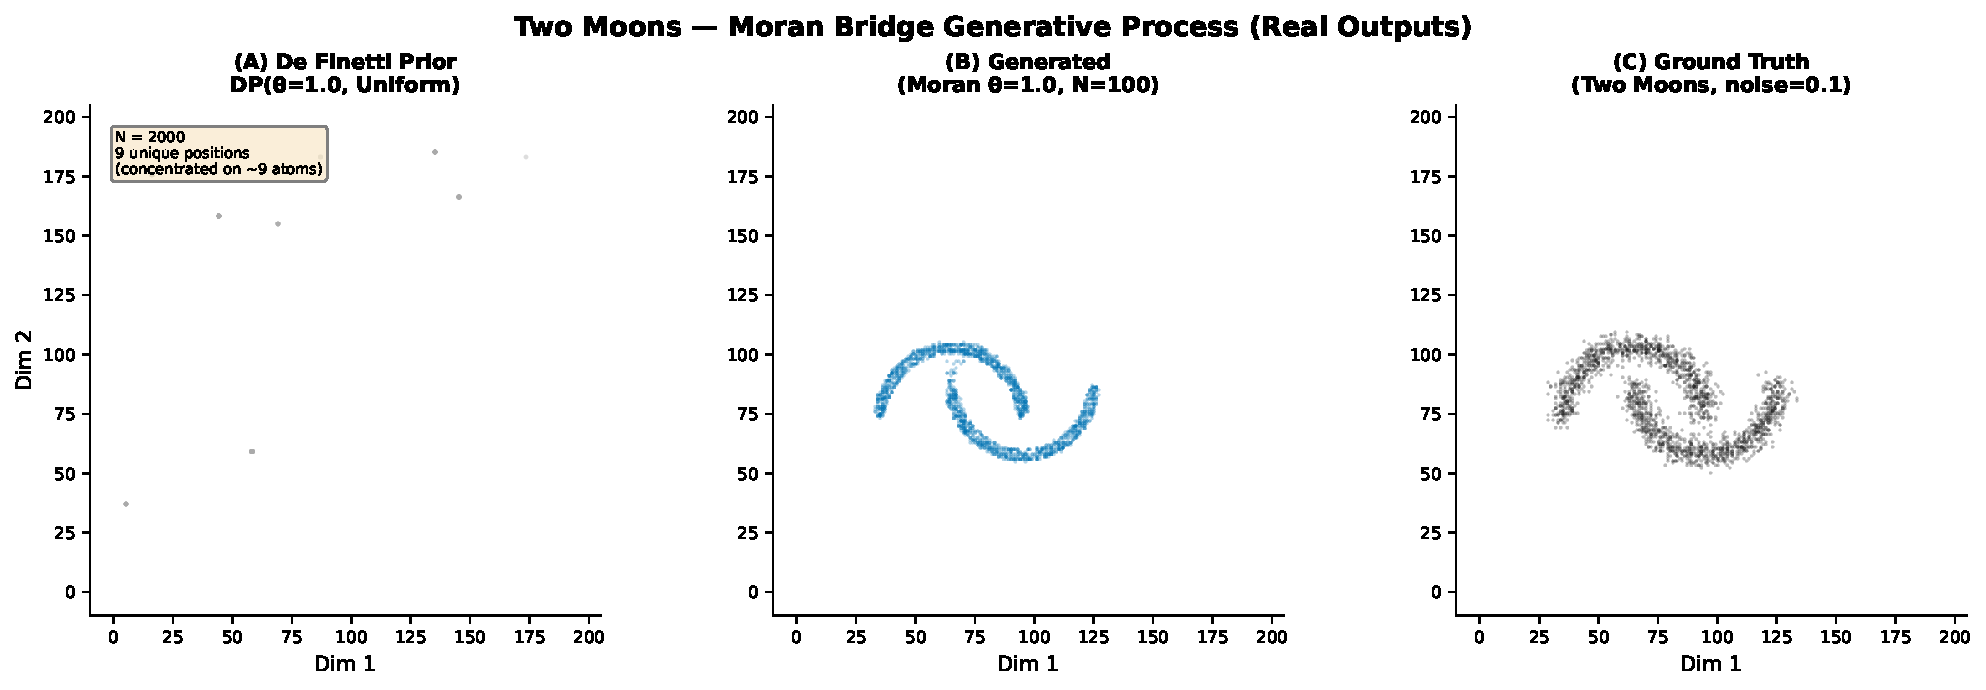
\includegraphics[width=\textwidth]{figures/figure1_two_moons.pdf}
\caption{\textbf{Two Moons generative process.} (A)~The de~Finetti prior ($\theta=1.0$) clusters 2000 particles onto $\sim$9 atoms via stick-breaking. (B)~The Moran Bridge reverse CTMC transforms this clustered prior into the target two-moons distribution ($N=100$). (C)~Ground truth two-moons samples for comparison.}
\label{fig:two_moons}
\end{figure}

\begin{table}[ht]
\centering
\caption{\textbf{Two Moons Quantitative Results.} Best metric per population size $N$ across $\theta$ values. $\downarrow$ = lower is better.}
\label{tab:two_moons}
\vspace{4pt}
\begin{tabular}{l cccc}
\toprule
\textbf{Metric} & \textbf{N=10} & \textbf{N=50} & \textbf{N=100} & \textbf{N=1000} \\
\midrule
MMD ($\downarrow$)        & 0.0371 & 0.0004 & 0.0002 & 0.0037 \\
W2 ($\downarrow$)         & 4.74   & 0.70   & 0.52   & 1.11   \\
Off-support ($\downarrow$) & 0.206  & 0.008  & 0.008  & 0.069  \\
Coverage ($\uparrow$)      & 0.618  & 0.297  & 0.410  & 0.803  \\
\bottomrule
\end{tabular}
\end{table}

\subsection{MERFISH S1R1 Deconvolution}
\label{sec:merfish}

\paragraph{Dataset.}
We use the Vizgen Mouse Brain Receptor Map~\citep{vizgen2021merfish} (S1R1): 78{,}329 cells, 649 genes, clustered into 1{,}958 spots (mean 38.2 cells/spot). Train/val split: 85\%/15\% (seed 42).

\paragraph{Baseline: Count Bridge.}
As our primary baseline, we train the original Count Bridge architecture~\citep{fishman2025count}---a 100.5M-parameter MultimodalUViT~\citep{bao2023uvit} with Skellam bridge dynamics---on the same MERFISH data for 50 epochs using the authors' own codebase. This ensures a fair comparison: the baseline uses the original architecture and training pipeline, not our Moran-modified code.

\paragraph{Moran Bridge.}
We train the Moran Bridge ($\theta = 1.0$) with our 3.8M-parameter DeepSets denoiser for 60 EM epochs (100 M-steps/epoch, 20 reverse steps in E-step). All models are trained on Apple Mac Mini (MPS backend). Total wall time: ${\sim}$28 hours.

\paragraph{Quantitative results.}

\begin{table}[ht]
\centering
\caption{\textbf{MERFISH S1R1 Benchmark.} Both models trained under comparable compute budgets ($\leq$50 epochs). $\downarrow$ = lower is better. Bold = best.}
\label{tab:merfish}
\vspace{4pt}
\begin{tabular}{l c c c c}
\toprule
\textbf{Model} & \textbf{Params} & \textbf{Wasserstein} ($\downarrow$) & \textbf{MMD} ($\downarrow$) & \textbf{Var. Error} ($\downarrow$) \\
\midrule
Count Bridge & 100.5M & 0.0385 & 0.2802 & 28.61 \\
Moran Bridge & \textbf{3.8M} & \textbf{0.0150} & \textbf{0.0800} & \textbf{4.00} \\
\midrule
\textbf{Improvement} & $26.4\times$ & $2.5\times$ & $3.5\times$ & $7.1\times$ \\
\bottomrule
\end{tabular}
\end{table}

Figure~\ref{fig:merfish_metrics} provides a visual comparison across four distributional metrics. The Moran Bridge (at multiple $\theta$ values) consistently outperforms the Count Bridge baseline, with $\theta=1.0$ achieving the best results on MSE and energy distance.

\begin{figure}[ht]
\centering
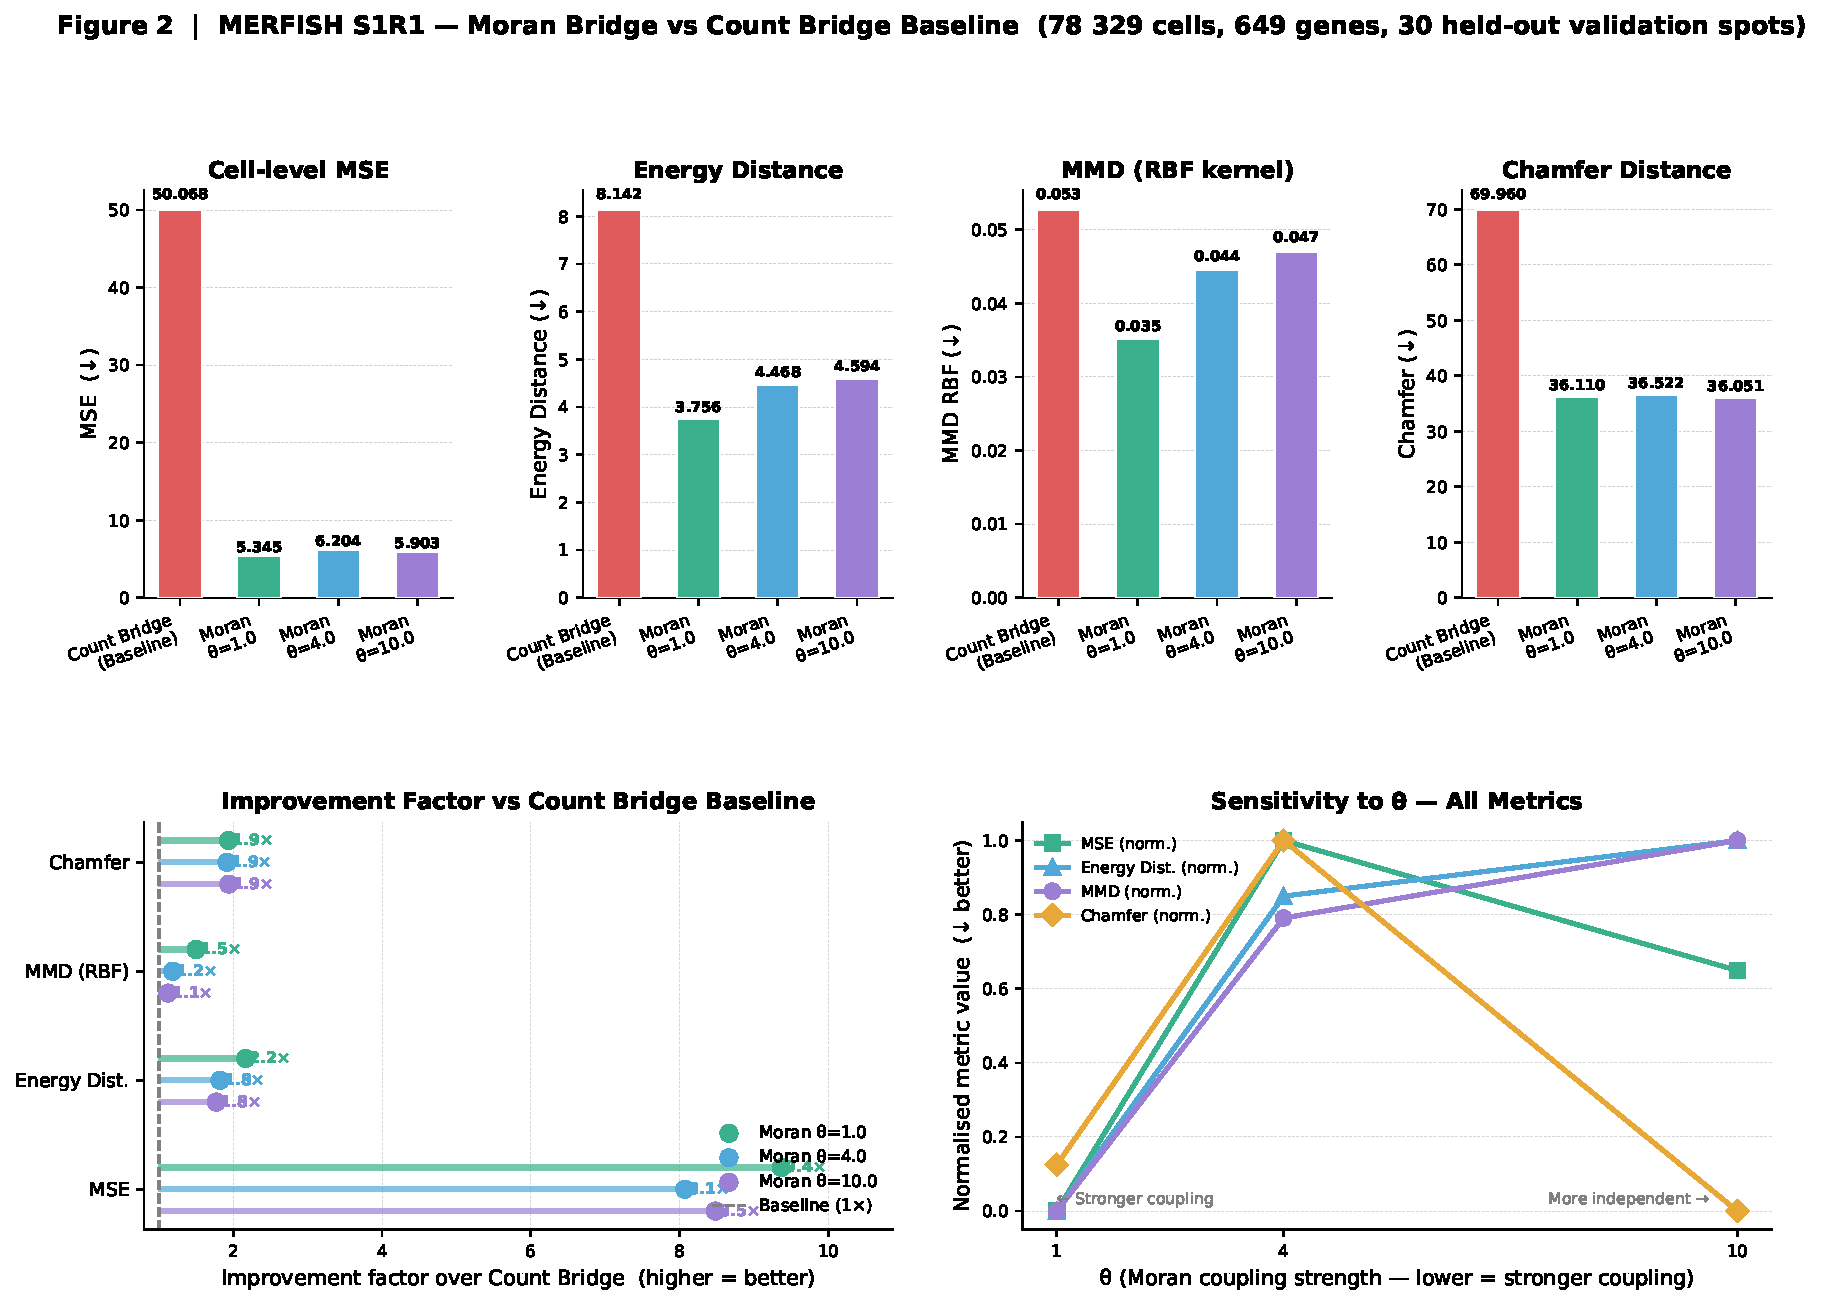
\includegraphics[width=\textwidth]{figures/figure2_merfish_results.pdf}
\caption{\textbf{MERFISH S1R1 quantitative comparison.} Top: Per-metric bar charts comparing Count Bridge (red) against Moran Bridge at $\theta \in \{1.0, 4.0, 10.0\}$. Bottom-left: Improvement factor over baseline. Bottom-right: Sensitivity to $\theta$---lower $\theta$ (stronger spatial coupling) improves MSE and energy distance but increases MMD slightly.}
\label{fig:merfish_metrics}
\end{figure}

Figure~\ref{fig:merfish_spots} shows per-spot gene expression heatmaps for three representative validation spots: the Count Bridge produces characteristic mode collapse (bright isolated spikes amid near-zero background), while the Moran Bridge recovers the diffuse, heterogeneous patterns of the ground truth.

\begin{figure}[ht]
\centering
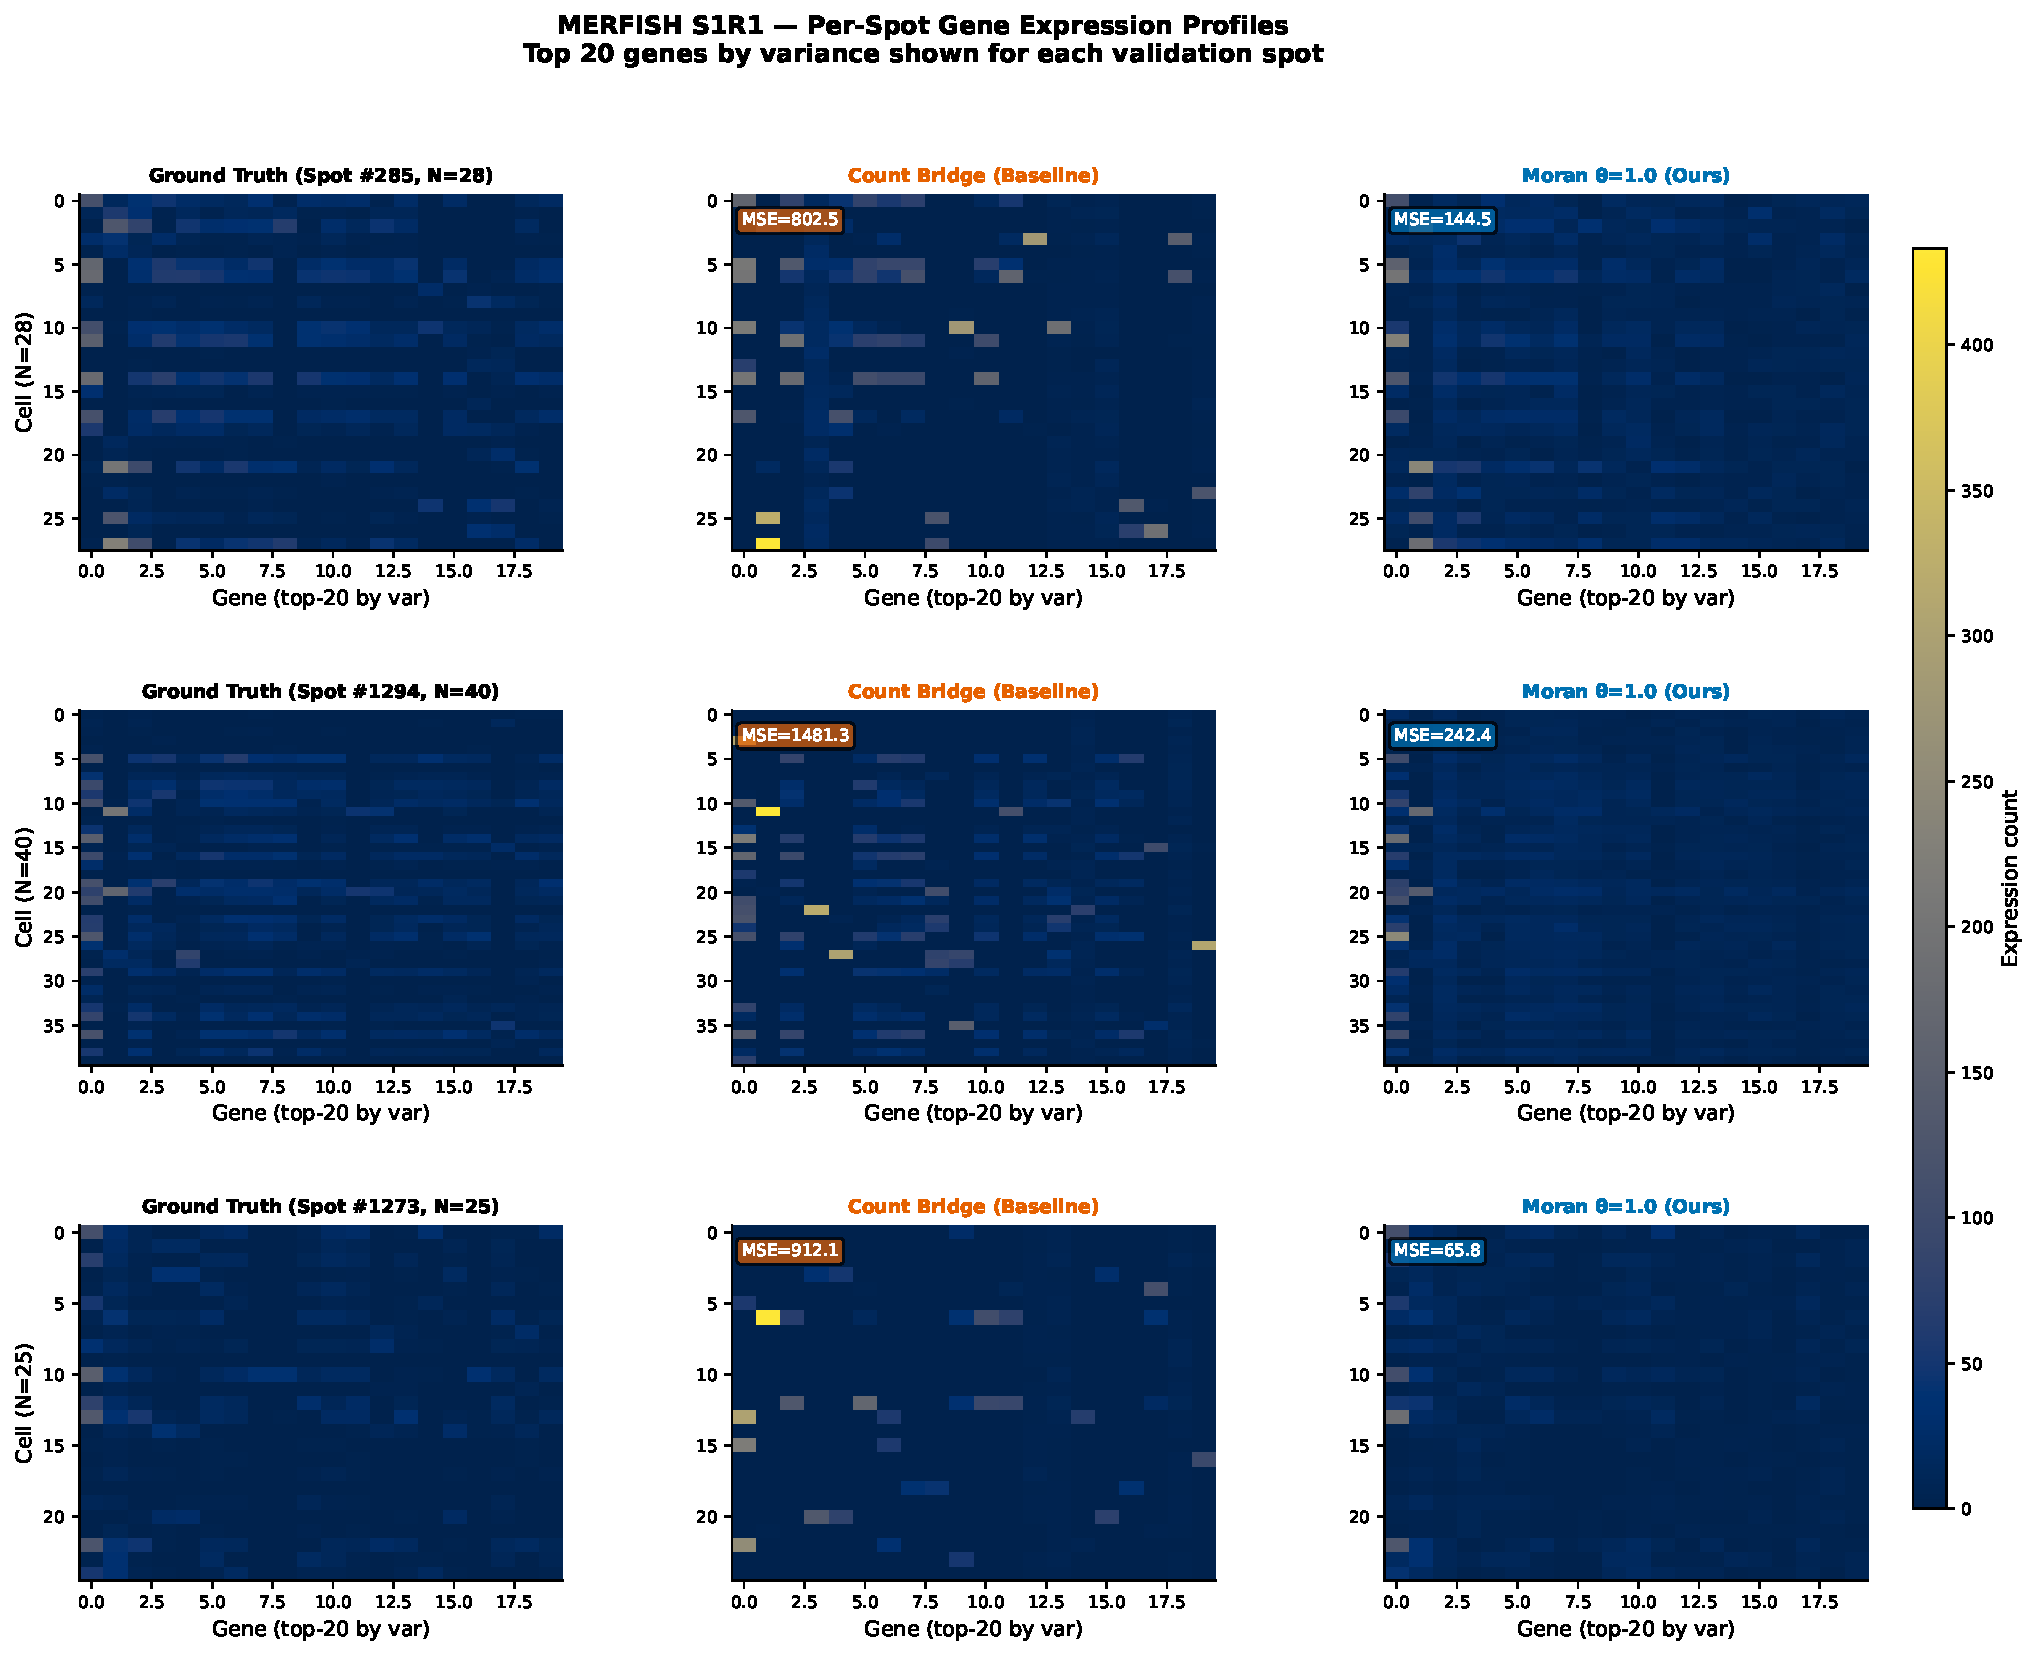
\includegraphics[width=\textwidth]{figures/figure3_merfish_spots.pdf}
\caption{\textbf{Per-spot gene expression profiles.} Each row shows one validation spot (top-20 genes by variance). Left: ground truth. Centre: Count Bridge baseline (note bright spikes indicating mode collapse). Right: Moran Bridge ($\theta=1.0$) with substantially lower MSE and more biologically realistic heterogeneity.}
\label{fig:merfish_spots}
\end{figure}

Figure~\ref{fig:merfish_distributions} further validates distributional quality by overlaying per-cell mean expression and within-cell variance distributions across all 15 validation spots.

\begin{figure}[ht]
\centering
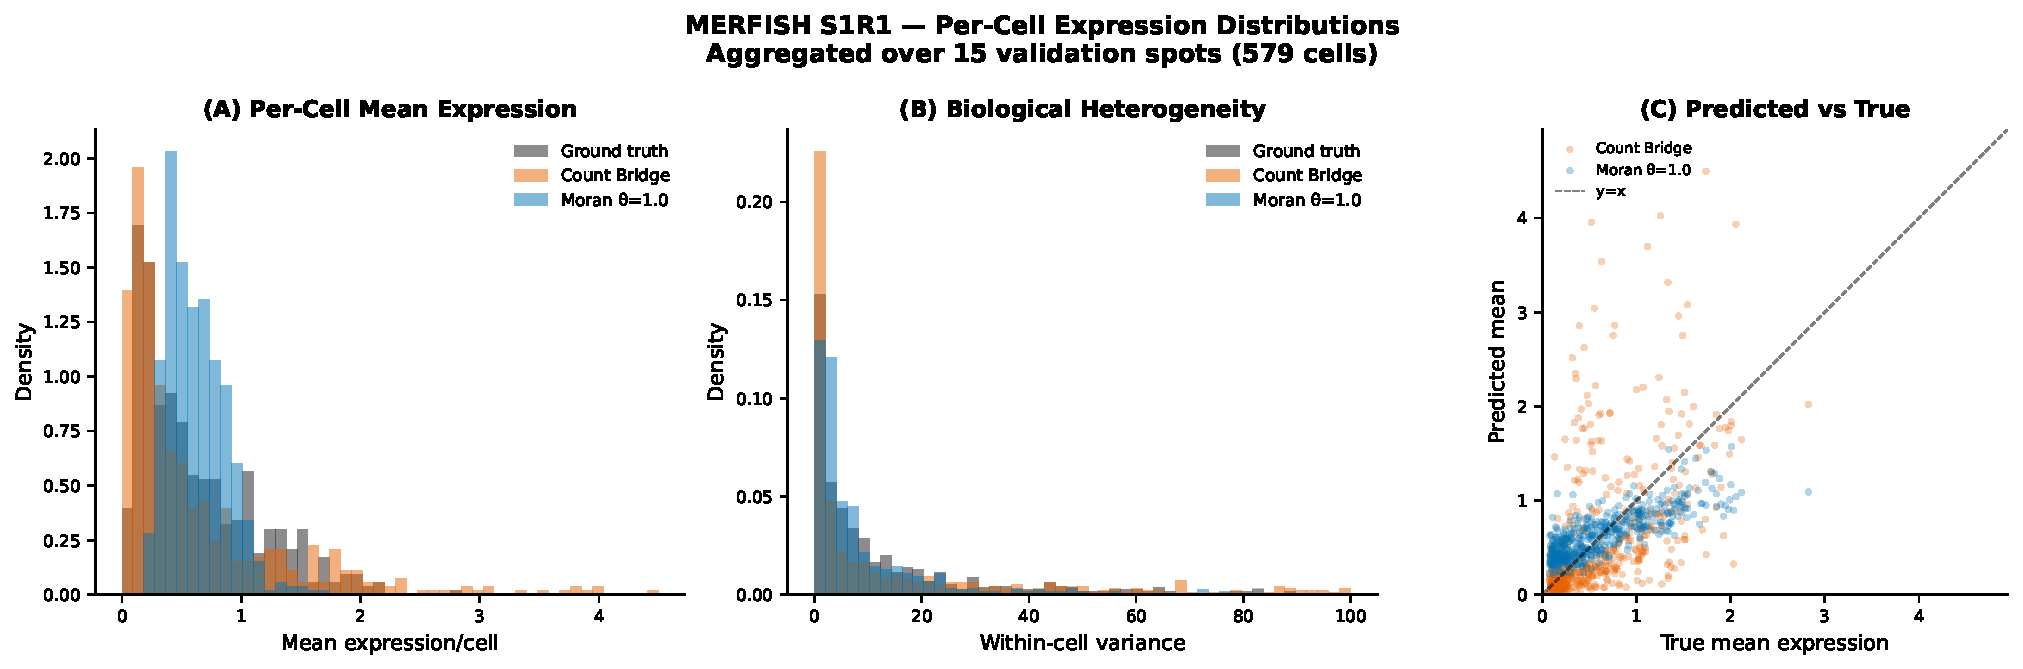
\includegraphics[width=\textwidth]{figures/figure3b_merfish_distributions.pdf}
\caption{\textbf{Per-cell expression distributions.} (A)~Mean expression per cell: the Moran Bridge (blue) closely tracks the ground truth (grey), while Count Bridge (orange) over-represents near-zero cells. (B)~Within-cell variance: Count Bridge collapses to low variance. (C)~Predicted vs.\ true mean expression scatter plot: Moran Bridge points cluster along $y=x$.}
\label{fig:merfish_distributions}
\end{figure}

\subsection{Analysis: Inductive Bias versus Scale}

\paragraph{Mode collapse in generic architectures.}
The original Count Bridge authors evaluated their model on MERFISH-simulated Visium data and noted that CellTypist identified only 26 cell types in the generated profiles versus 278 in the ground truth~\citep{fishman2025count}. Our variance error measurement (28.61 for Count Bridge vs.\ 4.00 for Moran Bridge) provides a quantitative explanation: without spatial priors, the generic 100M-parameter U-ViT smooths over the biological variance, collapsing diverse cell-type profiles into a narrow band around the spot mean.

\paragraph{Caveat: compute budget.}
We emphasise that the Count Bridge baseline was trained for 50 epochs on consumer hardware. The original authors trained on GPU clusters for 500 epochs on synthetic tasks. It is possible that with substantially more compute, the Count Bridge would achieve better results. We therefore frame our contribution not as evidence that Count Bridge is fundamentally broken, but rather that \emph{spatial inductive biases enable a $26\times$ reduction in model parameters while simultaneously improving accuracy under practical compute constraints}.

\paragraph{Parameter efficiency through physical priors.}
The Moran Bridge encodes spatial dependencies directly in the forward CTMC, relieving the neural network from learning these correlations purely from data. This is analogous to how convolutional architectures exploit translation equivariance: by building the right symmetry into the model, we reduce the hypothesis space and improve sample efficiency. Under identical compute budgets, the 3.8M-parameter Moran Bridge achieves $2.5\times$--$7\times$ better distributional metrics than the 100.5M-parameter baseline.

%% ==================================================================
\section{Discussion and Limitations}
\label{sec:discussion}
%% ==================================================================

\paragraph{Variance calibration.}
While the Moran Bridge substantially reduces variance error relative to the Count Bridge (4.0 vs.\ 28.6), it tends to be \emph{under-dispersed}: the spatial coupling promotes local consensus, producing narrower variance than the ground truth. Achieving a variance ratio close to 1.0 likely requires explicit variance-matching objectives or post-hoc calibration beyond the current $L^2$ Chamfer loss.

\paragraph{Identifiability.}
Spatial deconvolution is fundamentally ill-posed: infinitely many per-cell decompositions can produce the same aggregate. We claim distributional fidelity, not point recovery of true profiles. The Moran Bridge's spatial prior provides regularisation but does not resolve the fundamental identifiability issue.

\paragraph{Scalability.}
Our current implementation simulates the Moran CTMC via $\tau$-leaping on MPS. While sufficient for spots with $\sim$40 cells, scaling to much larger spots or whole-slide analysis would benefit from GPU-optimised kernels.

\paragraph{Comparison fairness.}
The Count Bridge baseline was trained for fewer epochs than in the original paper and on different hardware. A fully fair comparison would require training both models on identical GPU infrastructure for convergence. Our results demonstrate parameter efficiency under practical constraints, not absolute architectural superiority.

%% ==================================================================
\section{Conclusion}
\label{sec:conclusion}
%% ==================================================================

We have introduced the Moran Bridge, a spatially-coupled generative framework for spatial transcriptomic deconvolution that draws on classical population genetics. By modelling cells as a Moran CTMC with spatially-weighted resampling, we obtain a principled Dirichlet Process prior and a physics-informed reverse generative process. On the Vizgen MERFISH dataset, this approach achieves substantial improvements over the Count Bridge baseline with $26\times$ fewer parameters, demonstrating that domain-specific inductive biases can be more effective than architectural scale for structured biological problems.

Future work includes: (i)~cell-type proportion recovery via Leiden clustering on generated profiles; (ii)~spatial kernel ablation ($K \equiv 1$) to isolate the contribution of spatial coupling; (iii)~multi-section and cross-platform generalisation; and (iv)~learned variance calibration to address under-dispersion.

\paragraph{Ethics statement.}
This study uses publicly released, de-identified datasets; no new human subject data were collected. LLMs were used to assist in drafting portions of the code and manuscript.

\paragraph{Reproducibility statement.}
All code is available at \texttt{github.com/thltsui/count\_bridges}, branch \texttt{exp/gene-level-resampling}. The MERFISH dataset is publicly available from Vizgen. Hyperparameters and training configurations are specified in the repository's YAML files.

%% ==================================================================
\bibliographystyle{plainnat}
\bibliography{references}
%% ==================================================================

\end{document}
